% !TEX program = xelatex
\documentclass[a4paper]{article}
\usepackage{amsmath}
\usepackage{amsthm}
\usepackage[left=1.8cm,right=1.8cm,top=2.2cm,bottom=2.0cm]{geometry}
\usepackage{ctex}
\usepackage{enumerate}
\usepackage{fancyhdr}
\usepackage{xpatch}
\usepackage{graphicx} 
\usepackage{float} 
\usepackage{subfigure} 
\usepackage{amsfonts}
\usepackage{mathtools}
\usepackage{framed}
\usepackage{multicol}
\usepackage{minted}
\usepackage{hyperref}
\usepackage{biblatex}
\addbibresource{08-discussion.bib}
\usepackage{tikz}

\usetikzlibrary{automata,positioning}
\theoremstyle{definition}
\newtheorem*{solution*}{\textbf{Solution:}}
\newtheorem*{proof*}{\textbf{Proof:}}
\newtheorem{theorem}{Theorem}[subsection]
\newtheorem{definition}{Definition}[subsection]
\newtheorem{lemma}{Lemma}[subsection]
\makeatletter

\AtBeginDocument{\xpatchcmd{\@thm}{\thm@headpunct{.}}{\thm@headpunct{}}{}{}}
\makeatother

\pagestyle{fancy}
\renewcommand{\baselinestretch}{1.15}

\usepackage{paralist}
\let\itemize\compactitem
\let\enditemize\endcompactitem
\let\enumerate\compactenum
\let\endenumerate\endcompactenum
\let\description\compactdesc
\let\enddescription\endcompactdesc

% shorten footnote rule
\xpatchcmd\footnoterule
  {.4\columnwidth}
  {1in}
  {}{\fail}

\title{CS 131 Compilers: Discussion 8: Loop Optimizations}
\author{\textbf{杨易为}~~\textbf{吴凌云}~~\textbf{樊雨鑫} \\ \texttt{ \{yangyw,wuly2,fanyx\}@shanghaitech.edu.cn}}

\begin{document}
\maketitle
\section{Loop Optimizations}
Major optimizations of loops
\begin{enumerate}
    \item Loop invariant variable extrapolation Loop invariant variable motion
    \item Induction variable elimination
    \item Constant loop expansion Const Loop Expansion
\end{enumerate}
Loop Definition: a loop is a subset $S$ of nodes where:
\begin{enumerate}
    \item  $S$ is strongly connected:
\item For any two nodes in $S$, there is a path from one to the other using only nodes in $S$
\item There is a distinguished header node $h \in S$ such that there is no edge from a node outside $S$ to $S \backslash\{h\}$ \cite{cs153lec18}
\end{enumerate}
\begin{figure}[htbp]
  \centering
  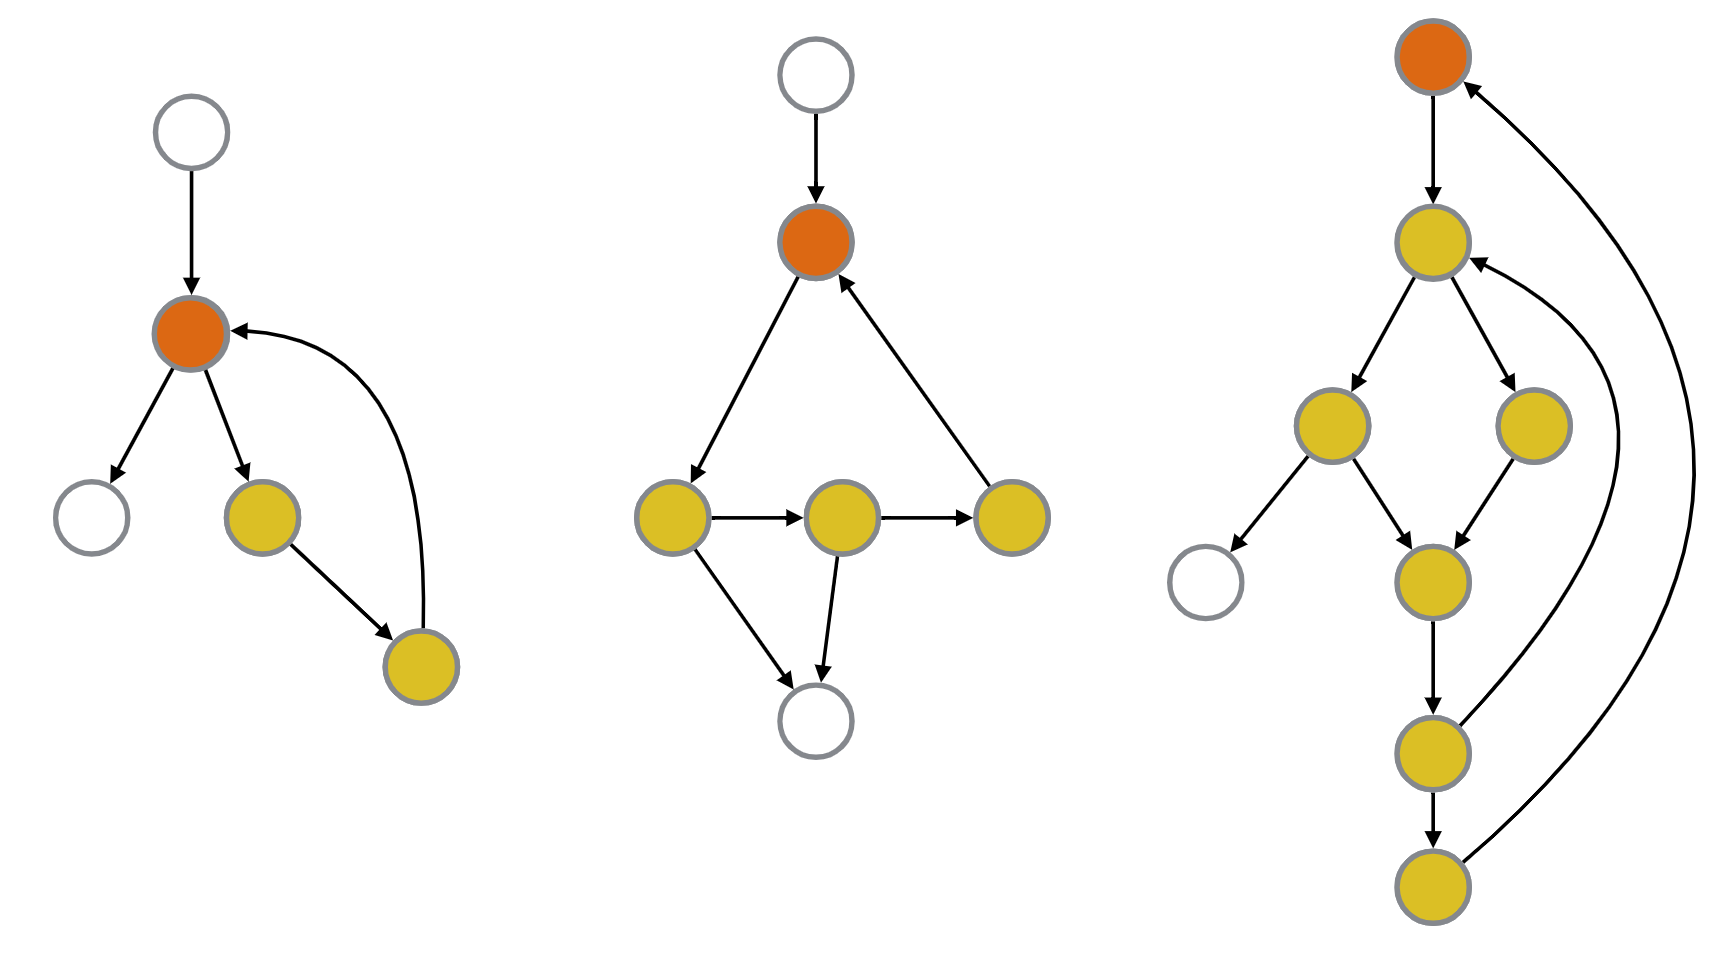
\includegraphics[width=10cm]{./img/loop_example.png}
  \caption{reducible graphs without gotos}
\end{figure}

To identify a loop:
\begin{enumerate}
    \item Only one entry point: header
\item There is at least one path to the header
\item Assume that there is a return edge n → header in the CFG and that the loop consists of n, header and all other nodes that do not need to go through header to reach n
\end{enumerate}

This definition is more formal and is actually the node between header and n, Further, a strongly connected component is a loop (except for size = 1)
A back edge is an edge that points to its ancestor in a depth-first search

To identify a nested loops
\begin{enumerate}
    \item If the header of two loops in a CFG is the same, then it is considered as one loop

\item If the header of the two loops in the CFG is different, then it is one of the following
\begin{enumerate}
\item The two loops do not intersect
\item One loop is contained within the other (inner and outer loops)
\end{enumerate}
\end{enumerate}
\subsection{LoopFind}
\begin{enumerate}
    \item  Definition: node $d$ dominates node $n$ if every path from the start node to $n$ must go through $d$
\item Definition: an edge from $n$ to a dominator $d$ is called a back-edge
\item Definition: a loop of a back edge $n \rightarrow d$ is the set of nodes $x$ such that $d$ dominates $x$ and there is a path from $x$ to $n$ not including $d$
\end{enumerate}
\begin{minted}[mathescape,linenos]{c}
void LoopFind::run() {
  std::unordered_set<CFGnode *> reserved;
  std::unordered_set<std::unordered_set<CFGnode *> *> comps;
  std::unordered_set<CFGnode *> nodes;
  for (auto func : m_->getFunctions()) {
    if (func->getBasicBlocks().size() == 0)
      continue;
    buildCFG(func, nodes);
    // Dominator logic
    while (stronglyConnComponents(nodes, comps)) {
    if (comps.size() == 0)
        break;
    for (auto set : comps) {
        auto base = findLoopBase(set, reserved);
        // store result
        auto BBset = new BBset_t;
        for (auto n : *set) {
          BBset->insert(n->BB);
        }
        loops.insert(BBset);
        base2Loop.insert({base->BB, BBset});
        loop2Base.insert({BBset, base->BB});
        for (auto BB : *BBset) {
          if (BB2Base.find(BB) == BB2Base.end())
            BB2Base.insert({BB, base->BB});
          else
            BB2Base[BB] = base->BB;
        }
    }
  }
}
\end{minted}
If loops $A$ and $B$ have distinct headers and all nodes in $B$ are in $A$ (i.e., $B \subseteq A$ ), then we say $B$ is nested within $A$

An inner loop is a nested loop that doesn't contain any other loops
\subsection{Loop Invariant\cite{15411lec17}}
An assignment $x:=v_{1}$ op $v_{2}$ is invariant for a loop if for each operand $v_{1}$ and $v_{2}$ either
\begin{enumerate}
    \item the operand is constant
    \item all of the definitions that reach the assignment are outside the loop
    \item only one definition reaches the assignment and it is a loop invariant
\end{enumerate}
\begin{minted}[mathescape,linenos]{c}
void LoopInvariant::run() {
  finder = std::make_unique<LoopFind>(m_);
  finder->run();
  areaCount = 0;
  for (auto it = finder->begin(); it != finder->end(); it++) {
    if (!finder->isBaseLoop(*it))
      continue;
    auto loop = *it;
    do {
      invariant.clear();
      findInvariants(loop);
      if (invariant.size())
        moveInvariantsOut(loop);
      loop = finder->getParentLoop(loop);
    } while (loop);
  }
}
\end{minted}
Before:
\begin{minted}[mathescape,linenos]{c}
L0: t := 0
 a := x
L1: i := i + 1
 b := 7
 t := a + b 
 *i := t 
 if i<N goto L1 else L2
L2:
 x := t
\end{minted}
After:
\begin{minted}[mathescape,linenos]{c}
L0: t := 0
  t := a + b 
L1: i := i + 1 
  *i := t 
  if i<N goto L1 else L2
L2: x := t
\end{minted}
False Negative: Although t’s definition is loop invariant, the *i is variant and live after the loop.
\begin{minted}[mathescape,linenos]{c}
L0: t := 0
L1: i := i + 1 
  *i := t // FN
if i<N goto L1 else L2
L2: x := t 
  t := a + b
\end{minted}
\begin{enumerate}
    \item 循环优化的收益按照循环的level指数放大,所以要辨识出inner loop
\item 局部性原理与循环transform(SIMD拓展
\end{enumerate}
\subsection{Loop unrolling}
Reduce the time between code start-up and wind-down.
\begin{figure}[htbp]
  \centering
  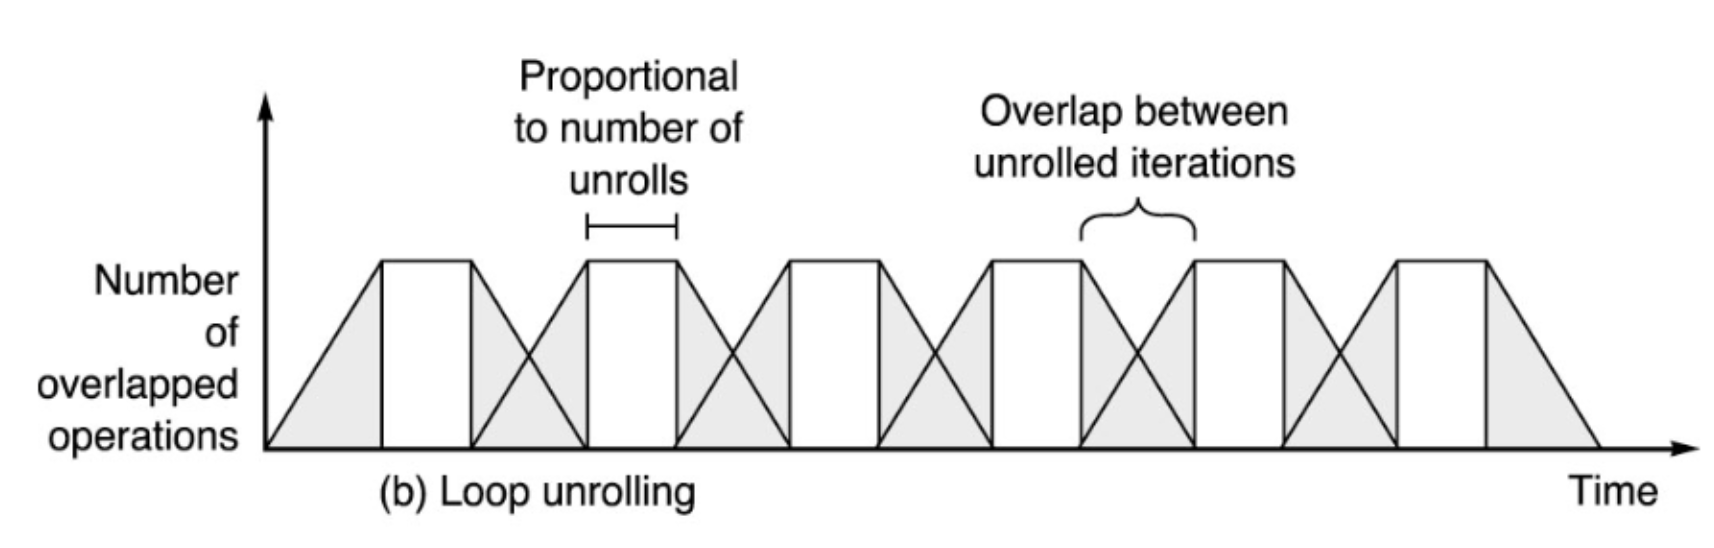
\includegraphics[width=10cm]{./img/loop_unroll.png}
\end{figure}
Before:
\begin{minted}[mathescape,linenos]{c}
for (int i = 0; i < n; ++i) { a[i] = b[i] * 7 + c[i] / 13;}
\end{minted}
After:
\begin{minted}[mathescape,linenos]{c}
for (int i = 0; i < n % 3; ++i) {
   a[i] = b[i] * 7 + c[i] / 13;
}
for (; i < n; i += 3) { 
   a[i] = b[i] * 7 + c[i] / 13;
   a[i + 1] = b[i + 1] * 7 + c[i + 1] / 13; 
   a[i + 2] = b[i + 2] * 7 + c[i + 2] / 13;
}
\end{minted}
\begin{enumerate}
    \item + Reduce branching penalty, end-of-loop-test costs 
    \item - Size of program increased
\end{enumerate}
\subsection{Detecting Induction Variables and Reduction}
%TODO
\begin{minted}[mathescape,linenos]{c}
s := 0 
i := 0
L1:
 if i >= n goto L2 
 j := i*4   
 k := j+a 
 x := *k 
 s := s+x  
 i := i+1
L2: ...
\end{minted}
\begin{enumerate}
    \item Note that i only changes by the same amount each iteration of the loop 
    \item We say that i is a linear induction variable
    \item It’s easy to express the change in j and k
    
    - Since j = 4*i + 0 and k = 4*i + a, if i changes by c, j and k change by 4*c
\end{enumerate}

Step 1:
\begin{minted}[mathescape,linenos]{c}
s := 0 
i := 0
j’:= 0 
k’:= a
L1:
  if i >= n goto L2 
  j := j’    
  k := k’
  x := *k  
  s := s+x  
  i := i+1
  j’:= j’+4 
  k’:= k’+4
L2: ... 
\end{minted}
Step 2: Dead code elimination
\begin{minted}[mathescape,linenos]{c}
s := 0 
i := 0
k’:= a
L1:
  if i >= n goto L2 
  x := *k'
  s := s+x  
  i := i+1 // Useless, too
  k’:= k’+4
L2: ... 
\end{minted}
Step 3: Stronger Dead code elimination
\begin{minted}[mathescape,linenos]{c}
s := 0 
k’:= a
L1:
  if k' >= 4 * n + a goto L2 
  x := *k'
  s := s+x  
  k’:= k’+4
L2: ... 
\end{minted}
\subsection{Loop fusion}
Before:
\begin{minted}[mathescape,linenos]{c}
int acc = 0;
for (int i = 0; i < n; ++i) { 
   acc += a[i]; a[i] = acc;
} 
for (int i = 0; i < n; ++i) { b[i] += a[i];}
\end{minted}
After:
\begin{minted}[mathescape,linenos]{c}
int acc = 0;
for (int i = 0; i < n; ++i) { 
   acc += a[i];
   a[i] = acc;
   b[i] += acc;
}
\end{minted}
\begin{enumerate}
    \item + No multiple loop startup.
    \item - may lose locality reference
\end{enumerate}
\subsection{Loop fission}
Reverse of ubove.
\subsection{Loop peeling}
Split first (or last) few iterations from loop and perform them separately.
Before:
\begin{minted}[mathescape,linenos]{c}
for (int i = 0; i < n; ++i) { b[i] = (i == 0) ? a[i] : a[i] + b[i-1];}
\end{minted}
After:
\begin{minted}[mathescape,linenos]{c}
b[0] = a[0];
for (int i = 1; i < n; ++i) { b[i] = a[i] + b[i-1];}
\end{minted}
\subsection{Loop interchange}
Change order of loop iteration variables
Before:
\begin{minted}[mathescape,linenos]{c}
for (int j = 0; j < n; ++j) { 
  for (int i = 0; i < n; ++i) {    
    a[i][j] += 1;  
}}
\end{minted}
After:
\begin{minted}[mathescape,linenos]{c}
for (int i = 0; i < n; ++i) {
  for (int j = 0; j < n; ++j) {
    a[i][j] += 1;
}}
\end{minted}
\subsection{Loop tiling}
For nested loop:
\begin{figure}[htbp]
  \centering
  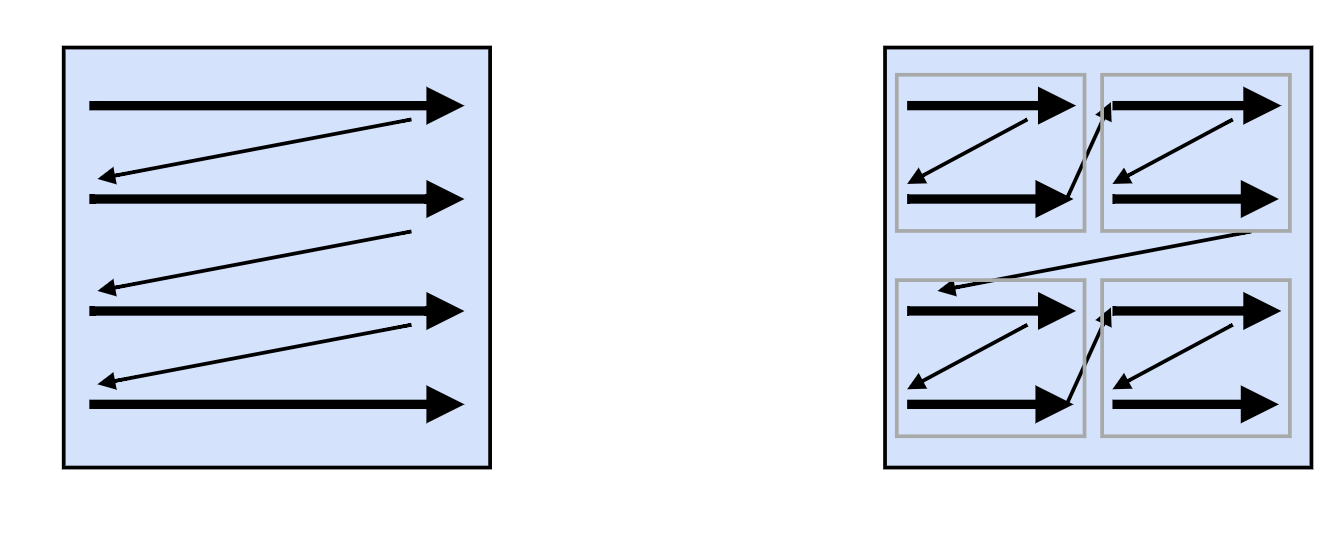
\includegraphics[width=10cm]{./img/loop_tiling.png}
  \caption{\cite{cs211lec11}}
\end{figure}
Before:
\begin{minted}[mathescape,linenos]{c}
for (i = 0; i < n; i++) {  
   c[i] = 0;
   for (j = 0; j < n; j++) {
        c[i] = c[i] + a[i][j] * b[j];  
   }
}
\end{minted}
After:
\begin{minted}[mathescape,linenos]{c}
for (i = 0; i < n; i += 4) {
    c[i] = 0;    
    c[i + 1] = 0;    
    for (j = 0; j < n; j += 4) {      
        for (x = i; x < min(i + 4, n); x++) {        
            for (y = j; y < min(j + 4, n); y++) {        
                c[x] = c[x] + a[x][y] * b[y];   
            }     
        } 
    }  
}
\end{minted}
\subsection{Software Pipelining}
\begin{figure}[htbp]
  \centering
  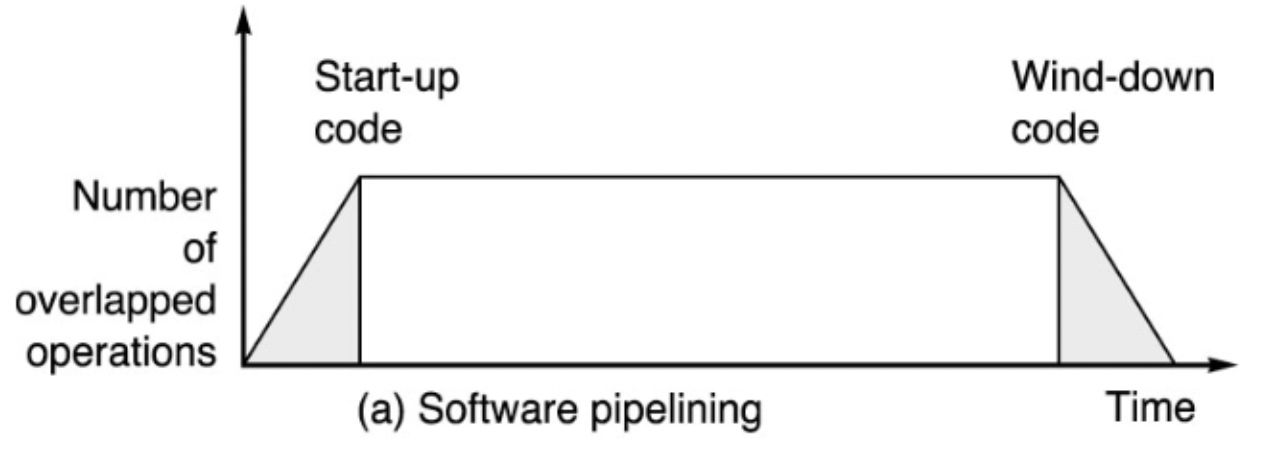
\includegraphics[width=10cm]{./img/sw_pipeline.png}
\end{figure}
Before:
\begin{minted}[mathescape,linenos]{c}
for i = 1 to bignumber
  A(i)
  B(i)
  C(i)
end
\end{minted}
After:
\begin{minted}[mathescape,linenos]{c}
for i = 1 to (bignumber - 2) step 3
  A(i)
  A(i+1)
  A(i+2)
  B(i)
  B(i+1)
  B(i+2)
  C(i)
  C(i+1)
  C(i+2)
end
\end{minted}
\section{Instruction Refactor}
\begin{enumerate}
    \item 融合比较和分支指令



Fuse之前:
\begin{minted}[mathescape,linenos]{llvm}
i1 %5  = CmpLT i32 %4 i32 100 
Br i1 %5 <label> %6 <label> %21
\end{minted}
Fuse之后
\begin{minted}[mathescape,linenos]{llvm}
Br LT i32 %4 i32 100 <label> %6 <label> %21 
省掉了一个寄存器 %5
\end{minted}
\begin{minted}[mathescape,linenos]{llvm}
1c1
< >>>>>>>>>>>> After pass 17DeadCodeEliminate <<<<<<<<<<<<
---
> >>>>>>>>>>>> After pass 7LowerIR <<<<<<<<<<<<
20,21c20
<     i1 %5  = CmpGT i32 %18 i32 1073741824 
<     Br i1 %5 <label> %6 <label> %10 
---
>     Br GT i32 %18 i32 1073741824 <label> %6 <label> %10 
29,30c28
<     i1 %12  = CmpLT i32 %19 i32 0 
<     Br i1 %12 <label> %13 <label> %16 
---
>     Br LT i32 %19 i32 0 <label> %13 <label> %16 
\end{minted}
\item 融合加法和乘法

这利用ARM的一项指令集的特色:将位移(shift)和回转(rotate)等功能并成"资料处理"型指令(算数、逻辑、和寄存器之间的搬移),举例来说,一个C语言的叙述(a可能是一个数组的地址)
\begin{minted}[mathescape,linenos]{c}
a = a + (j << 2);
\end{minted}
在ARM之下,可简化成只需一个word和一个cycle即可完成的指令
\begin{minted}[mathescape,linenos]{llvm}
ADD     Ra, Ra, Rj, LSL #2
\end{minted}
举例来说
\begin{minted}[mathescape,linenos]{llvm}
@ i32 %24  = Load [ 100 x i32]* %35 i32 %36 i32 2 
ldr r3, [r1, +r0, lsl #2]
\end{minted}
\end{enumerate}
\printbibliography
\end{document}
